\subsubsection{01.10.2015}
	\textit{\textbf{Time frame:}} 17:00-21:30 \newline
	\textit{\textbf{Preview:}} The purpose for this meeting was creating structural layout of the robot in CAD Creo Parametric 3.0.\newline \newline
  \textit{\textbf{Detailed explaination:}}
  \begin{enumerate}
  	\item We made a structural model of the robot. The whole construction was divided into particular modules. They are:
  	\begin{enumerate}
  		\item Chassis - carrying base and wheels mounted on it.
  		
  		\item Bucket - container for debris.
  		
  		\item Elevator - mechanism for lifting bucket.
  		
  		\item Gripper - mechanism for collecting debris.
  		
  		\item MSA - mechanism for scoring autonomus alpinists.
  	\end{enumerate}
  	\begin{figure}[H]
  		\begin{minipage}[h]{1\linewidth}
  			\center{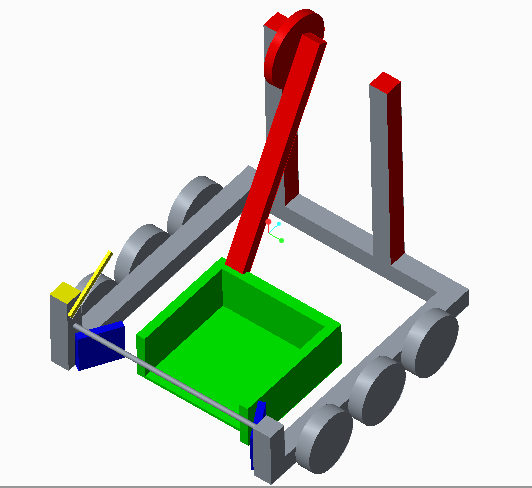
\includegraphics[scale=0.7]{days_L/01.10.2015/images/01}}
  			\caption{Schematic model of the robot}
  		\end{minipage}
  	\end{figure}
  	
  \end{enumerate}
  
   \newline
  \textit{\textbf{Additional comments:}} The task for the next meeting is to summarize our ideas for each module.

\fillpage
